\documentclass[
30pt,%font size
a1paper, 
landscape,% landscape or portrait
margin = 0mm,
innermargin = -2cm,
colspace = 5mm,
subcolspace = 0mm,
blockverticalspace=.5cm %spacing between blocks
]{tikzposter}
\usepackage[utf8]{inputenc}
\usepackage{geometry}
\geometry{paperwidth = 24in, paperheight = 36in}
 
\title{Improving Laser Guide Stars through Magnetic Resonant Pulsing}
\author{Adam Wright, Dr. Michaela Kleinert}
\date{\today}
\institute{Department of Physics, Willamette University, Salem, OR 97301}
 
\usepackage{comment}
\usepackage{graphicx}
\usepackage{tikz}
\usepackage{wrapfig,kantlipsum}


% Removes inscription at bottom right hand side of poster ``later tikzposter''
\tikzposterlatexaffectionproofoff

 
%%%%%%%%%%%%%%%%%%%%%%%%%%%%%%%%%%%%%%%%%%%%%%%%%%
% Block Style
%%%%%%%%%%%%%%%%%%%%%%%%%%%%%%%%%%%%%%%%%%%%%%%%%%

\defineblockstyle{sampleblockstyle}{
	titlewidthscale=1, bodywidthscale=1,titlecenter,
	titleoffsetx=0cm, titleoffsety=0pt, bodyoffsetx=0mm, bodyoffsety=15mm,
	bodyverticalshift=10mm, roundedcorners=5, linewidth=2pt,
	titleinnersep=6mm, bodyinnersep=1cm
}{
	\draw[color=framecolor, fill=blockbodybgcolor,
		rounded corners=\blockroundedcorners] (blockbody.south west)
		rectangle (blockbody.north east);
	\ifBlockHasTitle
		\draw[color=framecolor, fill=blocktitlebgcolor,
			rounded corners=\blockroundedcorners] (blocktitle.south west)
			rectangle (blocktitle.north east);
	\fi
}

\useblockstyle{sampleblockstyle}
%%%%%%%%%%%%%%%%%%%%%%%%%%%%%%%%%%%%%%%%%%%%%%%%%%
% colors
%%%%%%%%%%%%%%%%%%%%%%%%%%%%%%%%%%%%%%%%%%%%%%%%%%
\definecolorstyle{sampleColorStyle}{
	% Willamette Official Cardinal
	\definecolor{cardinal}{RGB}{121,23,22}
	% Willamette Official Gold
	\definecolor{gold}{RGB}{188,155,98}
	}{
	% Background Colors
	\colorlet{backgroundcolor}{white}
	\colorlet{framecolor}{white}
	% Title Colors
	\colorlet{titlefgcolor}{gold}
	\colorlet{titlebgcolor}{cardinal}
	% Block Colors
	\colorlet{blocktitlebgcolor}{cardinal}
	\colorlet{blocktitlefgcolor}{gold}
	\colorlet{blockbodybgcolor}{white}
	\colorlet{blockbodyfgcolor}{black}
	% Innerblock Colors
	\colorlet{innerblocktitlebgcolor}{white}
	\colorlet{innerblocktitlefgcolor}{black}
	\colorlet{innerblockbodybgcolor}{colorThree!30!white}
	\colorlet{innerblockbodyfgcolor}{black}
	% Note colors
	\colorlet{notefgcolor}{cardinal}
	\colorlet{notebgcolor}{cardinal}
    \colorlet{noteframecolor}{cardinal}}

%%%%%%%%%%%%%%%%%%%%%%%%%%%%%%%%%%%%%%%%%%%%%%%%%%
% Title layout
%%%%%%%%%%%%%%%%%%%%%%%%%%%%%%%%%%%%%%%%%%%%%%%%%%
\definetitlestyle{sampletitle}{
	width=1200mm,roundedcorners=20, linewidth=2pt, innersep=5pt,titletotopverticalspace=0mm, titletoblockverticalspace=10mm
}{
\begin{scope}[line width=\titlelinewidth, rounded corners=\titleroundedcorners]
	% Red box at top
	\draw[color=blocktitlebgcolor, fill=titlebgcolor]
		(\titleposleft,\titleposbottom) rectangle (\titleposright,\titlepostop);
	%Willamette Logo
	\node at (\titleposleft+150,\titleposbottom+125)
			{\includegraphics[scale = .75]{Images/compass.png}};
	% Lab Logo
	\node at (\titleposright-200,\titleposbottom+128)
			{\includegraphics[scale = 1.1]{Images/kleinertlogo.png}};
\end{scope}
}
 
% Using styles defined above
\usecolorstyle{sampleColorStyle}
\usetitlestyle{sampletitle}

%%%%%%%%%%%%%%%%%%%%%%%%%%%%%%%%%%%%%%%%%%%%%%%%%%
% Document Body
%%%%%%%%%%%%%%%%%%%%%%%%%%%%%%%%%%%%%%%%%%%%%%%%%%

\begin{document}
 
\maketitle

%%%%%%%%%%%%%%%%%%%%%%%%%%%%%%%%%%%%%%%%%%%%%%%%%%
% Create columns
%%%%%%%%%%%%%%%%%%%%%%%%%%%%%%%%%%%%%%%%%%%%%%%%%%
\begin{columns}
\centering
%%%%%%%%%%%%%%%%%%%%%%%%%%%%%%%%%%%%%%%%%%%%%%%%%%
% Create blocks in each column
%%%%%%%%%%%%%%%%%%%%%%%%%%%%%%%%%%%%%%%%%%%%%%%%%%

%%%%%%%%%%%%%%%%%%%%%%%%%%%%%%%%%%%%%%%%%%%%%%%%%%
% Column One
%%%%%%%%%%%%%%%%%%%%%%%%%%%%%%%%%%%%%%%%%%%%%%%%%%
    \column{0.3333}

	%%%%%%%%%%%%%%%%%%%%%%%%%%%%%%%%%%%%%%%%%%%%%%%%%%
	% Introduction
	%%%%%%%%%%%%%%%%%%%%%%%%%%%%%%%%%%%%%%%%%%%%%%%%%%
	
	\block{Introduction}
	{

\begin{wrapfigure}[8]{R}{0.55\linewidth}
	\begin{tikzfigure}[] 
			\includegraphics[width=0.13\textwidth]{Images/lgsvlt.png}
		\end{tikzfigure}
\end{wrapfigure}

Laser guide stars (LGS) are artificial stars created in Earth's atmosphere that aid in reducing blur from atmopheric distortion in telescopic imaging. Increasing the brightness of LGS improves the ability of the telescope system to reduce blur. Thus, LGS systems typically use high power laser beams. At high power, the polarization of light becomes an important factor in the LGS's brightness, and circular polarization creates the greatest brightness. However, this leads to optical pumping, which reduces the brightness due to the precession of atoms in the geomagnetic field. A solution to this is magnetic resonant pulsing (MRP).
	%Atoms with a magnetic moment $\vec \mu$ residing in a magnetic field $\vec B$ experience Larmor precession, a rotation of the atom’s total angular momentum vector about the axis of the magnetic field, with (Larmor) frequency $\omega_L = \gamma B$, where $\gamma$ is the gyromagnetic ratio. This precession degrades the benefits obtained through optical pumping, a technique used to increase atomic fluorescence.

	%We test \textit{Magnetic Resonant Pulsing} [MRP, Kane 2014], a technique that bypasses the consequences of Larmor precession and proposes to increases atomic fluorescence. MRP uses a laser pulsed at the Larmor frequency of the atom (a few hundred kHz in magnetic fields of less than a gauss), allowing light to interact with the atom at only one point in its precession cycle.

		%MRP has applications in optical magnetometry, atomic fluorescence, and laser guide stars, the motivation for this project. A laser guide star, shown in Figure \ref{fig:lgs}, is an artificial star created by shining laser light into the mesosphere where it is absorbed and emitted by sodium atom. This emission is useful for correcting telescopic images, which can be improved by increasing the brightness of the emission.
	}


	%%%%%%%%%%%%%%%%%%%%%%%%%%%%%%%%%%%%%%%%%%%%%%%%%%
	% Optical Pumping and MRP
	%%%%%%%%%%%%%%%%%%%%%%%%%%%%%%%%%%%%%%%%%%%%%%%%%%
	\block{Magnetic Resonant Pulsing}
	{

		\begin{minipage}{.15\textwidth}
			\vspace{-4cm}
		\begin{tikzfigure}[]
			\includegraphics[width=0.9\textwidth]{../Thesis/FullPaper/Images/tikz/opticalpumping.pdf}
		\end{tikzfigure}
		\end{minipage}
		\begin{minipage}{.15\textwidth}
			\begin{tikzfigure}[]
%			\vspace{-3cm}
			\includegraphics[width=0.8\textwidth]{Images/mrpangle.png}
		\end{tikzfigure}
		\end{minipage}

\begin{wrapfigure}[6]{r}{0.45\linewidth}
		\begin{tikzfigure}[]
			\vspace{1.5cm}
			\includegraphics[width=0.10\textwidth]{Images/precession.png}
		\end{tikzfigure}
\end{wrapfigure}
\vspace{-3cm}
The cycling transition normally established in the absence of a magnetic field is disrupted when the magnetic field is not parallel to the incoming light. This causes fluorescence to decrease as a non-optimal distribution of angular momentum occurs. By pulsing light at the Larmor frequency, the atom is essentially is not precessing with respect to the light, and the cycling transition is maintained.
%		Elliptically polarized light, $\sigma ^{\pm}$-polarized light requires the atom to transition to a state of greater projection number $m$ ($\Delta m = 1$) as shown in  Figure \ref{fig:opump}. While the decay allows for $\Delta m = \pm 1$, the following absorption again requires $\Delta m = 1$, which successively pushes the atoms to the stretched state. From there, the atom can only decay to a single state, thus resembling a two-level atom.

%\begin{wrapfigure}[9]{r}{0.5\linewidth}
%\end{wrapfigure}
%		This effect is very efficient when the magnetic field is parallel to the direction of the incident light; here, optical pumping greatly increases the fluorescence of atoms. However, as the angle between the laser and the magnetic field increases to $\pi$, fluorescence decreases significantly, shown via simulation in Figure \ref{fig:mrpangle} (blue curve) because the Larmor precession (Fig. 4) makes the cycling transition unattainable.

%		However, if the incoming light is pulsed at the Larmor frequency, light will only interact with the atom at one point in its precession cycle. Thus, to the light, the atom appears to not be precessing at all, and the cycling transition can be reestablished as shown in Fig. 3 (red curve).

	
	}

	%%%%%%%%%%%%%%%%%%%%%%%%%%%%%%%%%%%%%%%%%%%%%%%%%%
	% Second Column
	%%%%%%%%%%%%%%%%%%%%%%%%%%%%%%%%%%%%%%%%%%%%%%%%%%
    \column{0.3333}

		%%%%%%%%%%%%%%%%%%%%%%%%%%%%%%%%%%%%%%%%%%%%%%%%%%
		% Experimental aparatus
		%%%%%%%%%%%%%%%%%%%%%%%%%%%%%%%%%%%%%%%%%%%%%%%%%%
		\block{Experimental Set-up}
		{
			A pulsed laser was created with a diode laser ($\lambda = $ 780 nm) chopped by an acousto-optic modulator (AOM). The pulse width and repetition rate were controlled with a function generator connected to the AOM.
\begin{wrapfigure}[20]{R}{0.65\linewidth}
	\vspace{-2cm}
		\begin{tikzfigure}[]
			\includegraphics[width=0.15\textwidth]{Images/diodepulse.pdf}
		\end{tikzfigure}
		\begin{tikzfigure}[]
			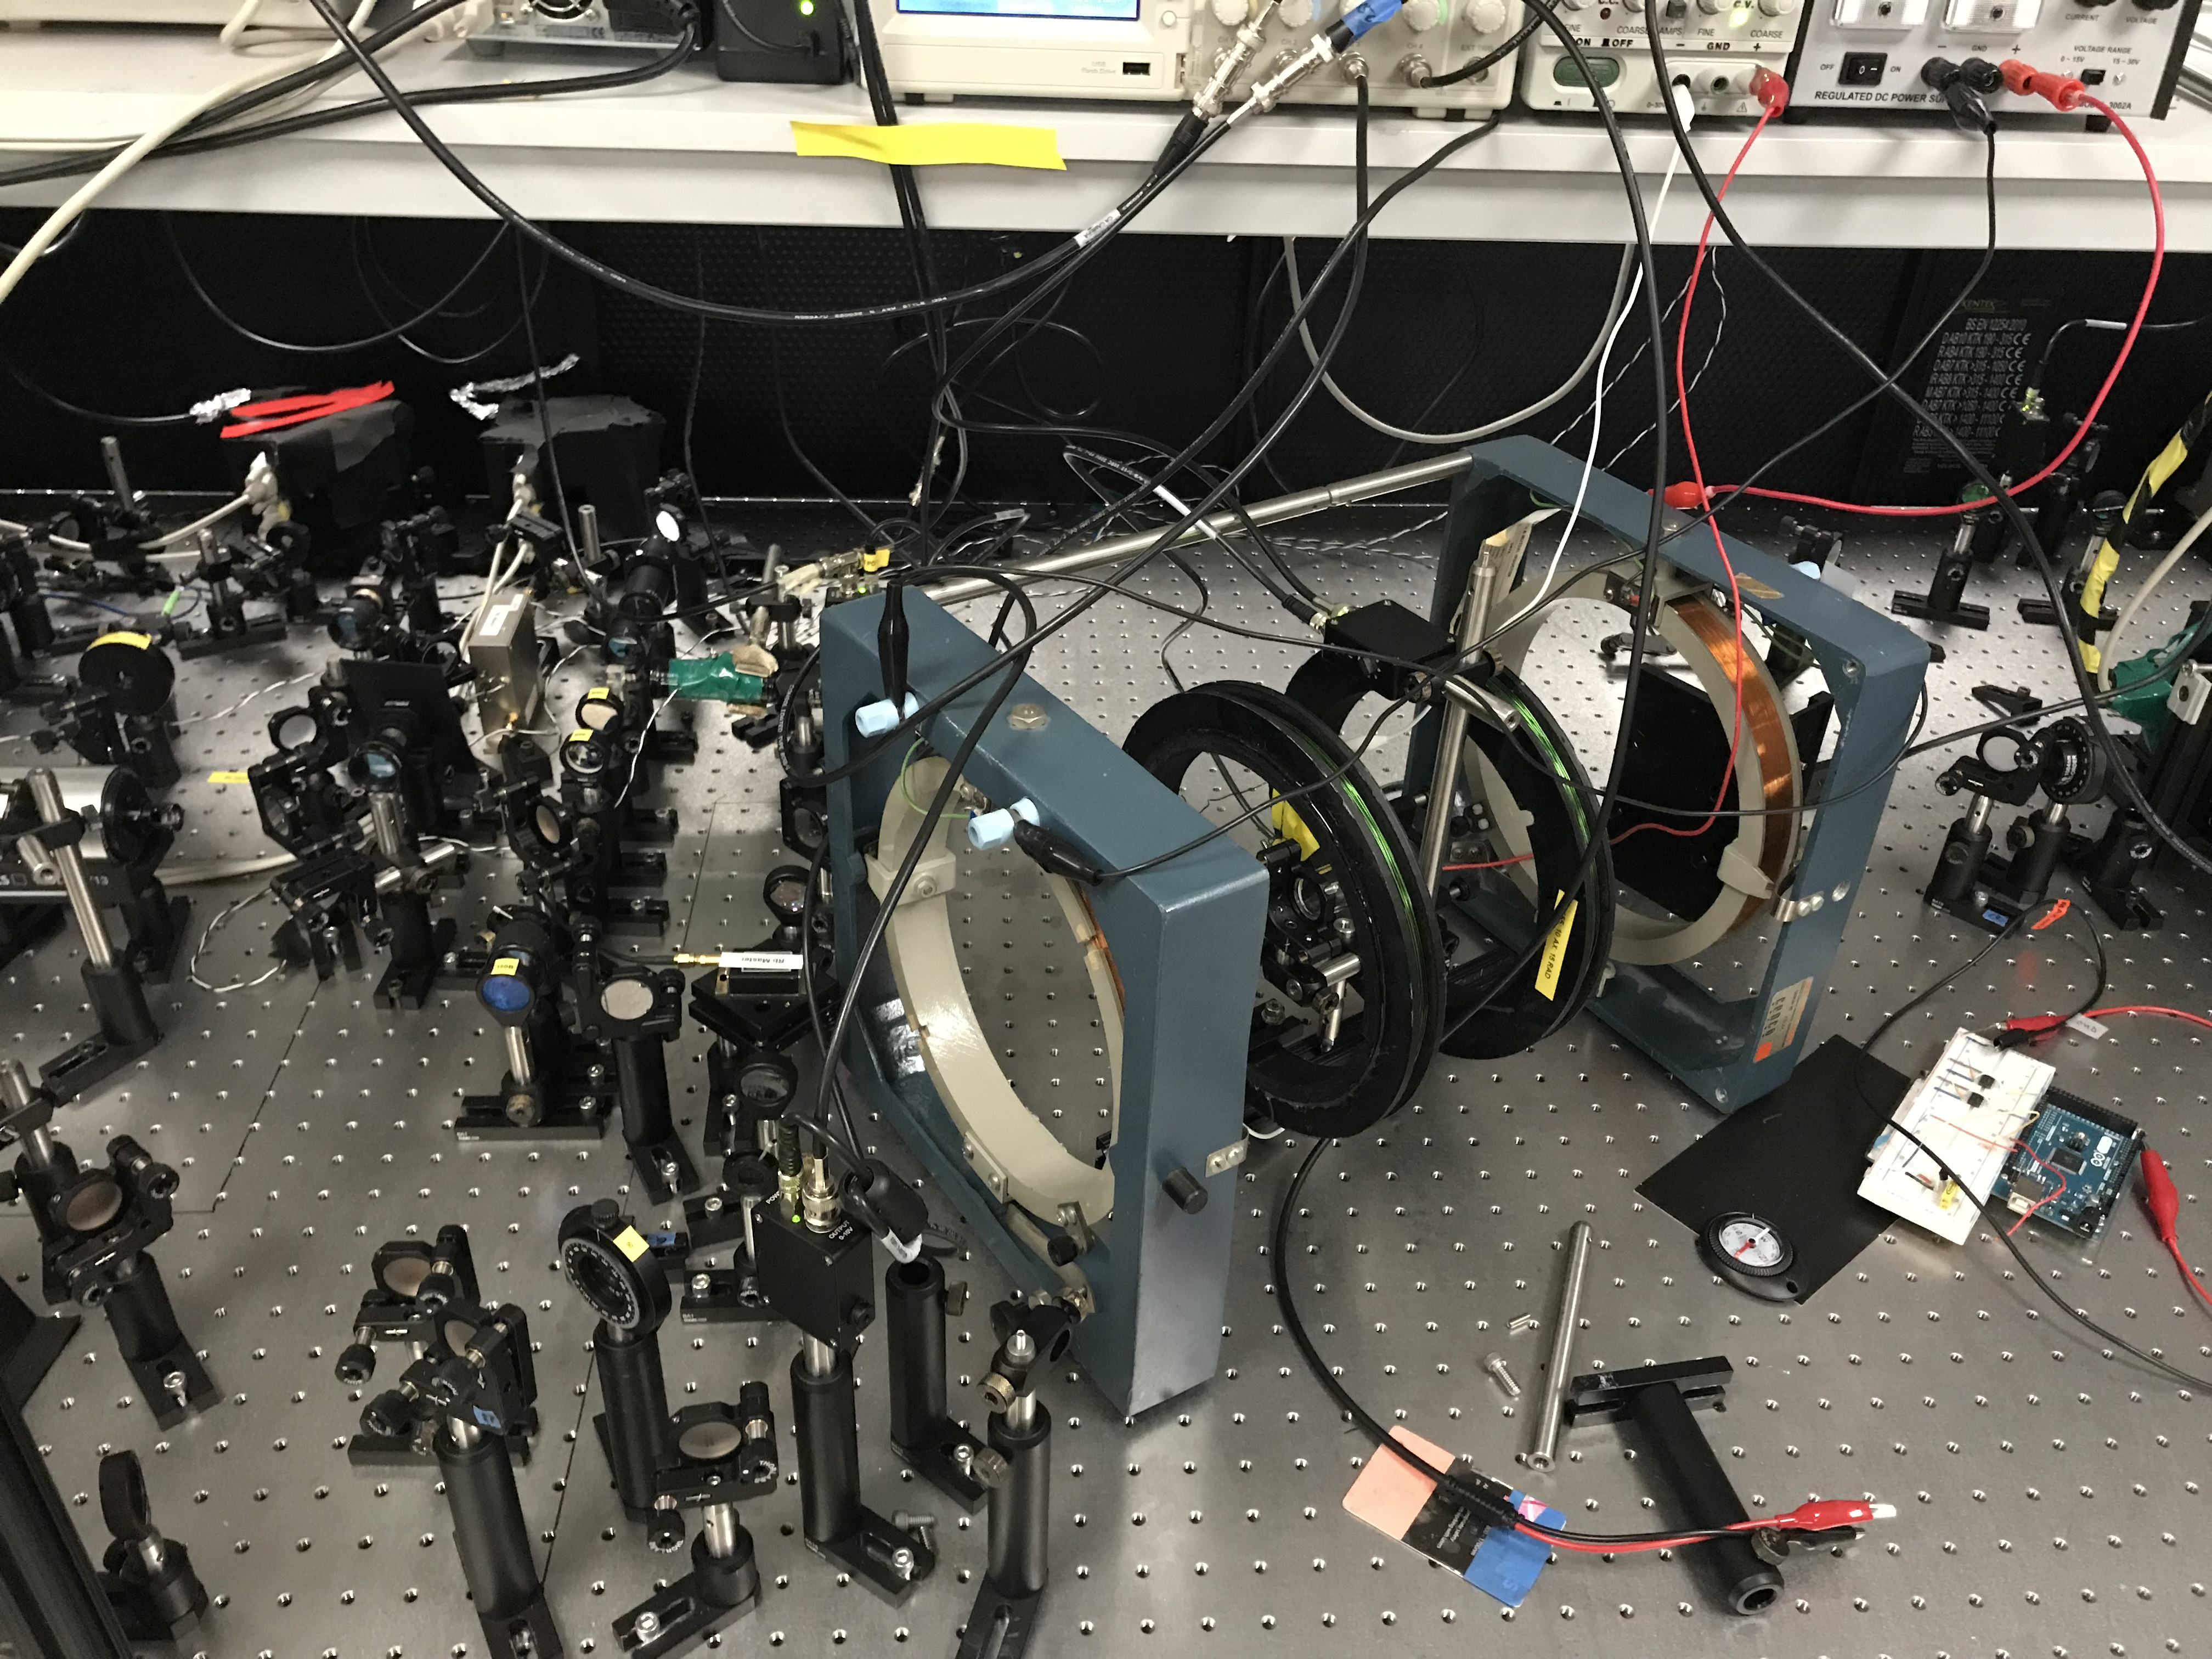
\includegraphics[width=0.15\textwidth]{Images/experiment.png}
		\end{tikzfigure}
	\end{wrapfigure}
		
		Two Helmholtz coil configurations were used, one to rid the system of external magnetic fields and the other to produce a constant magnetic field that could be rotated with respect to the laser beam. 
	The strength of the magnetic field inside the coils was measured as a function of position to ensure homogeneity within the system. 
	\vspace{1cm}
	
	
	\begin{minipage}{.15\textwidth}
		\begin{tikzfigure}[]
			\includegraphics[width=1\textwidth]{../Helmholtz/FieldAxial.png}
		\end{tikzfigure}
	\end{minipage}
	\begin{minipage}{.15\textwidth}
		\begin{tikzfigure}[]
			\includegraphics[width=1\textwidth]{../Helmholtz/FieldRadial.png}
		\end{tikzfigure}
		
	\end{minipage}
	
}
	%%%%%%%%%%%%%%%%%%%%%%%%%%%%%%%%%%%%%%%%%%%%%%%%%%
	% Third Column
	%%%%%%%%%%%%%%%%%%%%%%%%%%%%%%%%%%%%%%%%%%%%%%%%%%
	\column{.3333}

	%%%%%%%%%%%%%%%%%%%%%%%%%%%%%%%%%%%%%%%%%%%%%%%%%%
	% Data
	%%%%%%%%%%%%%%%%%%%%%%%%%%%%%%%%%%%%%%%%%%%%%%%%%%
	\block[]{Results}
	{
		A clear increase in fluorescence at the Larmor frequency can be seen when the magnetic field is perpendicular to the laser beam. The fluorescence of rubidium atoms is shown to stay constant over all magnetic field angles with a pulsed laser as opposed to decreasing with a continuous laser.\\
		\begin{minipage}{.15\textwidth}
			\begin{tikzfigure}[]
				\includegraphics[width=0.9\textwidth]{Images/FLvRep.pdf}
			\end{tikzfigure}
		\end{minipage}
		\begin{minipage}{.15\textwidth}
			\begin{tikzfigure}[]
			\includegraphics[width=0.9\textwidth]{../MRPData/April16/together.pdf}
		\end{tikzfigure}
		\end{minipage}
\\

		The percent change in fluorescence shows, for high intensity laser beams, that the fluorescence from continuous light decreases by roughly 30\% and, for low intensisites, 20\%. 

		\begin{minipage}{.15\textwidth}
		\begin{tikzfigure}[]
			\includegraphics[width=0.9\textwidth]{../MRPData/MAR24/togetherscaled.pdf}
		\end{tikzfigure}
		\end{minipage}
		\begin{minipage}{.15\textwidth}
		\begin{tikzfigure}[]
			\includegraphics[width=0.9\textwidth]{../MRPData/April16/togetherscaled.pdf}
		\end{tikzfigure}
		\end{minipage}


	}



	%%%%%%%%%%%%%%%%%%%%%%%%%%%%%%%%%%%%%%%%%%%%%%%%%%
	% Future Work
	%%%%%%%%%%%%%%%%%%%%%%%%%%%%%%%%%%%%%%%%%%%%%%%%%%
	\block{Future Work}
	{
		\begin{itemize}
			\item Look at using a repumping laser in order to counter the negative effects of downpumping present in the high intensity case. 
			\item Create pulsed laser with lower duty cycle, and find optimal duty cycle that results in highest fluorescence.
			%\item Create magnetic field shielding chamber in order to further eliminate external magnetic fields.
		\end{itemize}
		
	}
\end{columns}




%%%%%%%%%%%%%%%%%%%%%%%%%%%%%%%%%%%%%%%%%%%%%%%%%%
% References, contact information, funding
%%%%%%%%%%%%%%%%%%%%%%%%%%%%%%%%%%%%%%%%%%%%%%%%%%
\node [above right,
       outer sep=0pt,
       minimum width=\paperwidth-2*\pgflinewidth,
       minimum height=7cm,
       align=center,
       fill=cardinal,
	   text = gold] at ([shift={(0.5*\pgflinewidth,0.5*\pgflinewidth)}]bottomleft) 
	   {\textcolor{gold}{
	%Left Column
	\begin{minipage}{.15\textwidth}
		%%%%%%%%%%%%%%%%%%%%%%%%%%%%%%%%%%%%%%%%%%%%%%%%%%
		% Contact Information
		%%%%%%%%%%%%%%%%%%%%%%%%%%%%%%%%%%%%%%%%%%%%%%%%%%
		\LARGE
		\vspace{-1cm}
			Contact Information:\\
		\large
			Adam Newton Wright\\
			anwright@willamette.edu
	\end{minipage}
	% Center column
	\begin{minipage}{.55\textwidth}
		\LARGE References:
		\normalsize
		\begin{description}
			%%%%%%%%%%%%%%%%%%%%%%%%%%%%%%%%%%%%%%%%%%%%%%%%%%
			% You can put some references here
			%%%%%%%%%%%%%%%%%%%%%%%%%%%%%%%%%%%%%%%%%%%%%%%%%%
			\item ESO. Laser guide star at the VLT. https://www.eso.org/public/ images/dsc1792-cc/. Accessed: 4.12.2017.
			\item C. A. Denman, T. J. Kane, P. D. Hillman. Pulsed laser architecture for enhancing backscatter from sodium. International Society for Optics and Photonics, 9148:3G, 2014.
		\end{description}
	\end{minipage}
	%right column
	\begin{minipage}{.25\textwidth}
		\begin{minipage}{.25\textwidth}
			%%%%%%%%%%%%%%%%%%%%%%%%%%%%%%%%%%%%%%%%%%%%%%%%%%
			% NSF Logo or whatever you please
			%%%%%%%%%%%%%%%%%%%%%%%%%%%%%%%%%%%%%%%%%%%%%%%%%%
			\includegraphics{Images/nsf.png}
		\end{minipage}
		\begin{minipage}{.7\textwidth}
			%%%%%%%%%%%%%%%%%%%%%%%%%%%%%%%%%%%%%%%%%%%%%%%%%%
			% Whatever you need to say to please those who 
			% give you money $$$
			%%%%%%%%%%%%%%%%%%%%%%%%%%%%%%%%%%%%%%%%%%%%%%%%%%
			\large
			This work was supported by the National Science Foundation (grant \#1500376) and by Willamette University.
		\end{minipage}
	\end{minipage}
}
   };






%\colorlet{blocktitlebgcolor}{white}
%\colorlet{blockbodybgcolor}{cardinal}
%\colorlet{blockbodyfgcolor}{gold}
%\block[titleleft,titleoffsetx=2em,titleoffsety=1em,bodyoffsetx=2em,bodyoffsety=1em,titlewidthscale=1, bodywidthscale=1.03, roundedcorners=14,linewidth=6mm, bodyinnersep=10mm, titleinnersep=0mm]{}
%{
%	%Left Column
%	\begin{minipage}{.33\textwidth}
%		%%%%%%%%%%%%%%%%%%%%%%%%%%%%%%%%%%%%%%%%%%%%%%%%%%
%		% Contact Information
%		%%%%%%%%%%%%%%%%%%%%%%%%%%%%%%%%%%%%%%%%%%%%%%%%%%
%		Contact Information:\\
%		Adam Newton Wright\\
%		anwright@willamette.edu
%	\end{minipage}
%	% Center column
%	\begin{minipage}{.33\textwidth}
%		\begin{description}
%			%%%%%%%%%%%%%%%%%%%%%%%%%%%%%%%%%%%%%%%%%%%%%%%%%%
%			% You can put some references here
%			%%%%%%%%%%%%%%%%%%%%%%%%%%%%%%%%%%%%%%%%%%%%%%%%%%
%			\item Kane
%			\item Hillman...
%		\end{description}
%	\end{minipage}
%	%right column
%	\begin{minipage}{.33\textwidth}
%		\begin{minipage}{.15\textwidth}
%			%%%%%%%%%%%%%%%%%%%%%%%%%%%%%%%%%%%%%%%%%%%%%%%%%%
%			% NSF Logo or whatever you please
%			%%%%%%%%%%%%%%%%%%%%%%%%%%%%%%%%%%%%%%%%%%%%%%%%%%
%			\includegraphics{Images/nsf.png}
%		\end{minipage}
%		\begin{minipage}{.7\textwidth}
%			%%%%%%%%%%%%%%%%%%%%%%%%%%%%%%%%%%%%%%%%%%%%%%%%%%
%			% Whatever you need to say to please those who 
%			% give you money $$$
%			%%%%%%%%%%%%%%%%%%%%%%%%%%%%%%%%%%%%%%%%%%%%%%%%%%
%			This work was supported by this person and thenational science foundation and by many other people and I would like to thank them all for everything taht they have done for me and this research
%		\end{minipage}
%	\end{minipage}
%}
 
\end{document}
